\begin{enumerate}
    \item Explain precisely following abbreviations

	AS, RIP, OSPF, IGMP, EIGRP, ICMP, BGP, ARP, RARP, CIDR, DHCP, MTU
	
	\textbf{Answer:}
	
	\begin{itemize}
	    \item AS: An autonomous system (AS) is a collection of connected Internet Protocol (IP) routing prefixes under the control of one or more network operators on behalf of a single administrative entity or domain that presents a common, clearly defined routing policy to the Internet.
	    
	    \item RIP: The Routing Information Protocol (RIP) is one of the oldest distance-vector routing protocols which employ the hop count as a routing metric.
	    
	    \item OSPF: Open Shortest Path First (OSPF) is a routing protocol for Internet Protocol (IP) networks. It uses a link state routing (LSR) algorithm and falls into the group of interior gateway protocols (IGPs), operating within a single autonomous system (AS).
	    
	    \item IGMP: The Internet Group Management Protocol (IGMP) is a communications protocol used by hosts and adjacent routers on IPv4 networks to establish multicast group memberships. IGMP is an integral part of IP multicast.
	    
	    \item EIGRP: Enhanced Interior Gateway Routing Protocol (EIGRP) is an advanced distance-vector routing protocol that is used on a computer network for automating routing decisions and configuration.
	    
	    \item ICMP: The Internet Control Message Protocol (ICMP) is a supporting protocol in the Internet protocol suite. It is used by network devices, including routers, to send error messages and operational information indicating, for example, that a requested service is not available or that a host or router could not be reached.
	    
	    \item BGP: Border Gateway Protocol (BGP) is a standardized exterior gateway protocol designed to exchange routing and reachability information among autonomous systems (AS) on the Internet.
	    
	    \item ARP: The Address Resolution Protocol (ARP) is a communications protocol used for resolution of Internet layer addresses into link layer addresses, a critical function in the Internet protocol suite.
	    
	    \item RARP: The Reverse Address Resolution Protocol (RARP) is an obsolete computer networking protocol used by a client computer to request its Internet Protocol (IPv4) address from a computer network, when all it has available is its link layer or hardware address, such as a MAC address. The client broadcasts the request, and does not need prior knowledge of the network topology or the identities of servers capable of fulfilling its request.
	    
	    \item CIDR: Classless Inter-Domain Routing is a method for allocating IP addresses and IP routing. The Internet Engineering Task Force introduced CIDR in 1993 to replace the previous addressing architecture of classful network design in the Internet. Its goal was to slow the growth of routing tables on routers across the Internet, and to help slow the rapid exhaustion of IPv4 addresses.
	    
	    \item DHCP: The Dynamic Host Configuration Protocol (DHCP) is a standardized network protocol used on Internet Protocol (IP) networks. The DHCP is controlled by a DHCP server that dynamically distributes network configuration parameters, such as IP addresses, for interfaces and services.
	    
	    \item MTU: the maximum transmission unit (MTU) is the size of the largest network layer protocol data unit that can be communicated in a single network transaction.
	\end{itemize}

	\item Can ATM network provide QoS support? Why?
	
	\textbf{Answer: Yes.}
	
	ATM traffic contracts form part of the mechanism by which "quality of service" (QoS) is ensured. There are four basic types (and several variants) which each have a set of parameters describing the connection.

    \begin{enumerate}
        \item[CBR] Constant bit rate: a Peak Cell Rate (PCR) is specified, which is constant.
        \item[VBR] Variable bit rate: an average or Sustainable Cell Rate (SCR) is specified, which can peak at a certain level, a PCR, for a maximum interval before being problematic.
        \item[ABR] Available bit rate: a minimum guaranteed rate is specified.
        \item[UBR] Unspecified bit rate: traffic is allocated to all remaining transmission capacity.
    \end{enumerate}
    
    VBR has real-time and non-real-time variants, and serves for "bursty" traffic. Non-real-time is sometimes abbreviated to vbr-nrt.
	
	\item Which protocols does IP layer include?
	
	\textbf{Answer:}
	
	IPv4, IPv6, ICMP, IGMP, RIP
	
	\item Which features does IPv6 packet have?
	
	\textbf{Answer:}
	
	\begin{itemize}
	    \item Simple
	    \item Rich IP addresses
	\end{itemize}
	
	\item[P.10] Consider a datagram network using 8-bit host addresses. Suppose a router uses longest prefix matching and has the following forwarding table:
	
	\begin{tabular}{cc}
	    \hline
	    Prefix Match & Interface \\
	    \hline
	    1 & 0 \\
	    11 & 1 \\
	    111 & 2 \\
	    otherwise & 3 \\
	    \hline
	\end{tabular}
	
	For each of the four interfaces, give the associated range of destination host addresses and the number of addresses in the range.
	
	\textbf{Answer:}
	
	\begin{tabular}{c|cc}
	    Interface & Host Addresses Range & Number (Count) \\
	    \hline
	    0 & 128 - 191 & 64 \\
	    1 & 192 - 223 & 32 \\
	    2 & 224 - 255 & 32\\
	    3 & 0 - 127 & 128 \\
	\end{tabular}
	
	\item[P.22] Consider the following network. With the indicated link costs, use Dijkstra's shortest-path algorithm to compute the shortest path from x to all network nodes. Show how the algorithm works by computing a table.
    
    \begin{figure}[H]
        \centering
        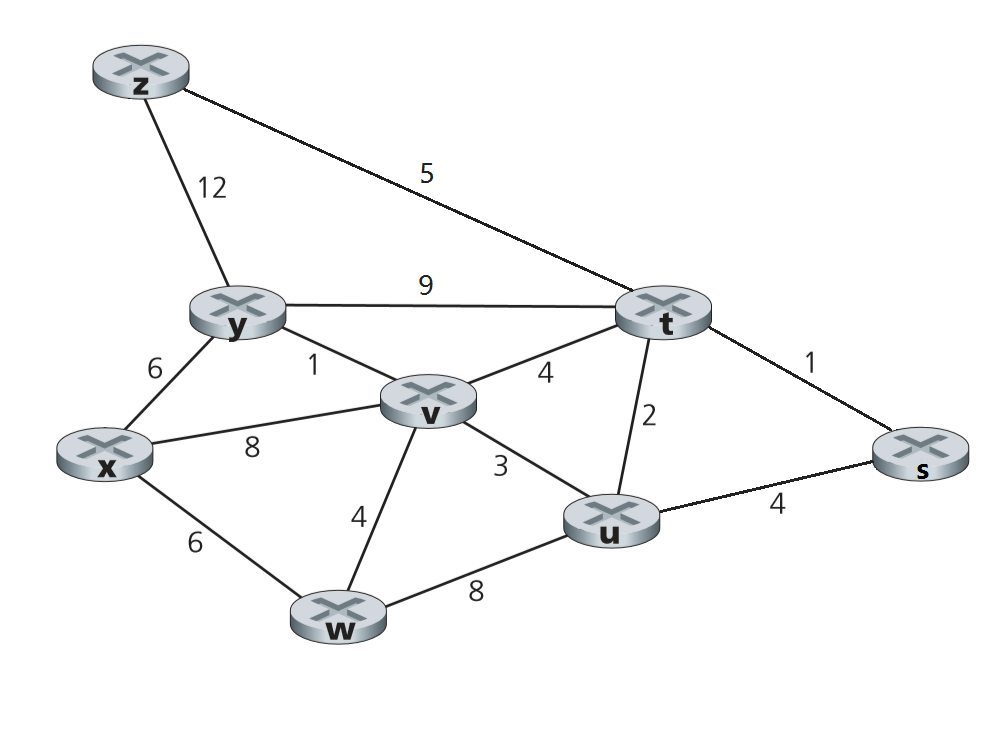
\includegraphics[width=0.8\textwidth]{4/P22.png}
        \caption{Network Topology}
        \label{fig:22}
    \end{figure}
    
    \textbf{Answer:}
	
	\begin{table}[H]
	    \centering
	    \begin{tabular}{ccccccccc}
	        \hline
	        step & N' & D(v),p(v) & D(w),p(w) & D(y),p(y) & D(u),p(u) & D(z),p(z) & D(t),p(t) & D(s),p(s) \\
	        \hline
	        0 & x & 8,v & 6,w & 6.y & $\infty$ & $\infty$ & $\infty$ & $\infty$ \\
	        1 & xy & 7,y & 6,w & & $\infty$ & 18,y & 15,y & $\infty$ \\
	        2 & xyw & 7,y & & & 14,w & 18,y & 15,y & $\infty$ \\
	        3 & xywv & & & & 10,y & 18,y & 11,y & $\infty$ \\
	        4 & xywvu & & & & & 18,y & 11,y & 14,y \\
	        5 & xywvut & & & & & 16,y & & 12,y \\
	        6 & xywvuts & & & & & 16,y & & \\
	        7 & xywvutsz & & & & & & & \\
	        \hline
	    \end{tabular}
	    \caption{Running the link-state algorithm on the network in Figure \ref{fig:22}}
	    \label{tab:4.3}
	\end{table}

	
	\item[P.25] Consider the network fragment shown below. $x$ has only two attached neighbors, $w$ and $y$. $w$ has a minimum-cost path to destination $u$ (not shown) of 5, and $y$ has a minimum-cost path to $u$ of 6. The complete paths from $w$ and $y$ to $u$ (and between $w$ and $y$) are not shown. All link costs in the network have strictly positive integer values.
	
    \begin{figure}[H]
        \centering
        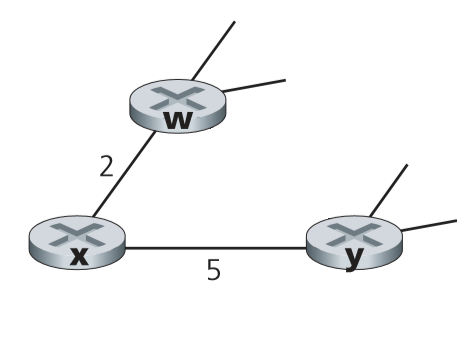
\includegraphics[width=0.3\textwidth]{4/P25.png}
    \end{figure}
	
	\begin{enumerate}[a.]
	    \item Give $x$'s distance vector for destinations $w$, $y$, and $u$.
	    
	    \textbf{Answer:}
	    
	    \begin{table}[H]
	        \centering
	        \begin{tabular}{c|ccc}
                \diagbox{from}{cost to} & w & y & u \\
                \hline
                w & 2 & 7 & 7 \\
                y & 7 & 5 & 11 \\
                \hline
                min & 2 & 5 & 7
	        \end{tabular}
	        \caption{Node x's DV}
	        \label{tab:xdv}
	    \end{table}
	    
	    \item Give a link-cost change for either $c(x, w)$ or $c(x, y)$ such that $x$ will inform its neighbors of a new minimum-cost path to $u$ as a result of executing the distance-vector algorithm.
	    
	    \textbf{Answer:}
	    
	    Decrease $c(x, w)$ to 1.
	    
	    \item Give a link-cost change for either $c(x, w)$ or $c(x, y)$ such that $x$ will not inform its neighbors of a new minimum-cost path to $u$ as a result of executing the distance-vector algorithm.
	    
	    \textbf{Answer:}
	    
	    Increase $c(x, y)$ to 6.
	    
	\end{enumerate}
	
	\item[P.31] Consider the following network. ISP B provides national backbone service to regional ISP A. ISP C provides national backbone service to regional ISP D. Each ISP consists of one AS. B and C peer with each other in two places using BGP. Consider traffic going from A to D. B would prefer to hand that traffic over to C on the West Coast (so that C would have to absorb the cost of carrying the traffic cross-country), while C would prefer to get the traffic via its East Coast peering point with B (so that B would have carried the traffic across the country). What BGP mechanism might C use, so that B would hand over A-to-D traffic at its East Coast peering point? To answer this question, you will need to dig into the BGP specification.
	
    \begin{figure}[H]
        \centering
        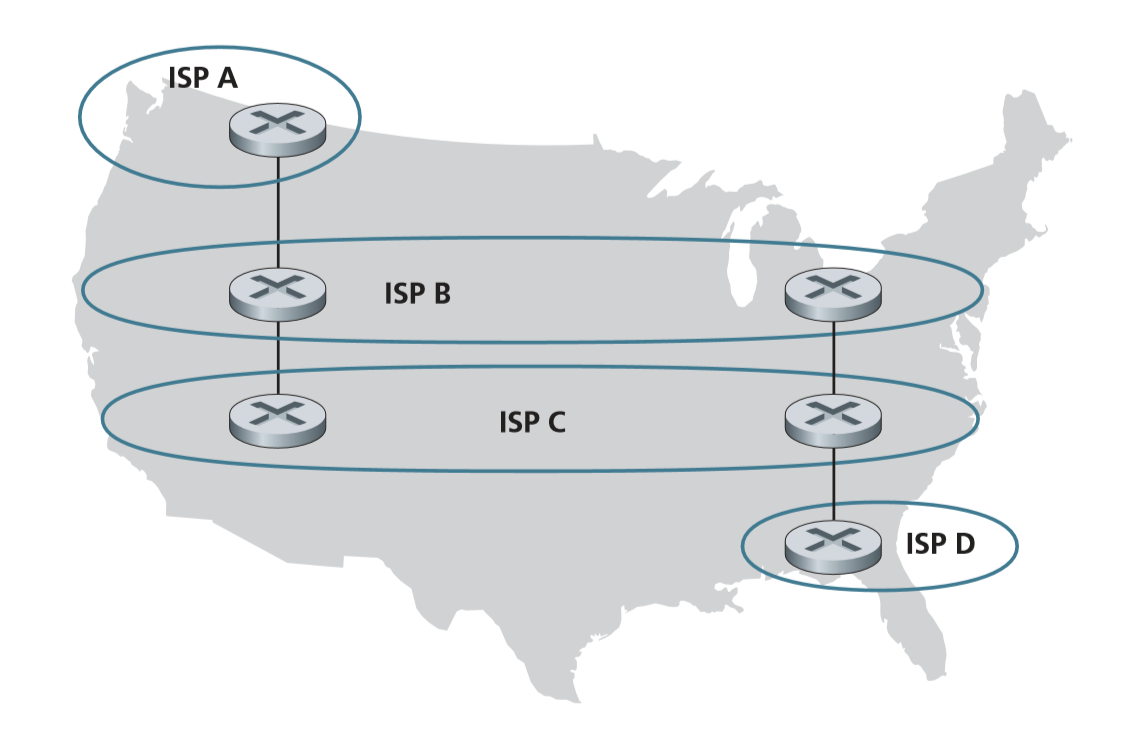
\includegraphics[width=0.8\textwidth]{4/P31.png}
    \end{figure}
    
    \textbf{Answer:}
    
    ISP C can send NOTIFICATION message to tell ISP B close the connection on the west coast.
	
	\item[P.35] Consider the two basic approaches identified for achieving broadcast, unicast emulation and network-layer (i.e., router-assisted) broadcast, and suppose spanning-tree broadcast is used to achieve network-layer broadcast. Consider a single sender and 64 receivers. Suppose the sender is connected to the receivers by a binary tree of routers. What is the cost of sending a broadcast packet, in the cases of unicast emulation and network-layer broadcast, for this topology? Here, each time a packet (or copy of a packet) is sent over a single link, it incurs a unit of cost. What topology for interconnecting the sender, receivers, and routers will bring the cost of unicast emulation and true network-layer broadcast as far apart as possible? You can choose as many routers as you'd like.
	
	\textbf{Answer:}
	
	\begin{enumerate}
	    \item Unicast Emulation
	    
	    The sender unicast the packet to 32 receivers, for each:
	    
	    The sender send a packet to root router, cost 1.
	    
	    The root router forward the packet to next router until next node is the receiver, cost 5.
	    
	    So unicast emulation cost 32 * (1 + 5) = 192.
	    
	    \item Network-layer broadcast.
	    	    
	    Router save and forward the packet, so each link will be only travelled once, cost $1 + 2 + 4 + \cdots + 32 = 63$.
	    
	\end{enumerate}
	
	To bring the cost of unicast emulation and true network-layer broadcast as far apart as possible, we should make the routes from sender to receivers have more common part. In the most special case, the topology is just like a broom in morphological.
	
	
\end{enumerate}